% Springer LNCS template, as required by AIPR 2026 (proceedings in LNCS).
% Compile with pdflatex + bibtex (splncs04). Overleaf: Menu -> Compiler: pdfLaTeX.
% AIPR 2026 sets no page limit for the manuscript (confirmed 2026-10-16). Working target about 20 pages.
\documentclass[runningheads]{llncs}

\usepackage[T1]{fontenc}
\usepackage{amsmath,amssymb}
\usepackage{graphicx}
\usepackage{booktabs}
\usepackage{xcolor}
\usepackage{tikz}
\usetikzlibrary{arrows.meta,positioning,fit,calc}
\usepackage{subcaption}
\usepackage{url}
\usepackage{listings}
\usepackage{siunitx}
\sisetup{detect-all}
\usepackage[hidelinks]{hyperref}
\renewcommand\UrlFont{\color{blue}\rmfamily}

% Draft markers. Delete this block before submission; no marker may remain.
\newcommand{\verify}[1]{\textcolor{red}{[VERIFY: #1]}}
\newcommand{\citeneeded}{\textcolor{red}{[CITATION NEEDED]}}

\lstset{basicstyle=\ttfamily\scriptsize, breaklines=true, columns=fullflexible, frame=single}

\graphicspath{{figures/}}

\begin{document}

\title{Ontology-Guided Appearance Variation of Egocentric Manipulation Video with World Foundation Models}
\titlerunning{Ontology-Guided Appearance Variation of Egocentric Video}

\author{Shrey Jha \and Skyler Saucedo \and Frank Tanner}
\authorrunning{S. Jha et al.}

\institute{Innodata Inc.\\
\email{xxx@innodata.com}}

\maketitle

\begin{abstract}
Vision-language-action policies are trained on tens of thousands to millions of demonstrations, and most of that volume exists to cover appearance: different counters, different buckets, different light. Recording that variety by hand in a household is slow. Domain randomization adds variety cheaply but without regard to the task, and recent video editing models can restyle a clip but offer no principled way to decide what should change or to keep the rest fixed. We describe a three-stage pipeline that addresses the first problem and measures how far current tools are from the second. A world foundation model (Cosmos 3 Nano) reads a 15-second egocentric clip and emits a task ontology: the action primitive, each task-relevant object with a bounding box, and candidate variations grounded in the object's role. A language model filters the candidates and writes a generation prompt. SAM2 converts boxes to tracked masks, and a subtraction step isolates the surface to be changed; edge, depth, blurred-RGB and segmentation controls then drive Cosmos Transfer 2.5. On 116 clips (about 30 min of footage) the reasoning stage proposes about 72 admissible variations per clip in 130 s, and a Transfer render takes 20 min on one A100; we rendered 64. The recolor succeeds where intended: the target region moves by a mean CIE76 $\Delta E$ of 75. It also moves the region it was told to preserve by 35, and 95\% of protected pixels change visibly. Action-level variation with Cosmos Predict2 produced no visible motion change. Appearance diversity is now cheap to propose and render; spatial containment and action generation are the open problems.

\keywords{Synthetic data \and World foundation models \and Video-to-video generation \and Egocentric video \and Robot learning \and Vision-language-action models.}
\end{abstract}


\section{Introduction}

A household robot that learns to wipe a counter from one recording will wipe that counter. Change the laminate from white to blue, swap the bucket, or move the task to a different kitchen, and a policy trained on the single clip has no reason to generalize. Vision-language-action (VLA) models such as RT-2~\cite{rt2}, OpenVLA~\cite{openvla} and $\pi_0$~\cite{pi0} get around this by training on very large demonstration sets~\cite{oxe}, and a large share of that scale is spent on appearance rather than on new skills. Collecting appearance diversity by hand is the slow part. Our source material for this work is 8 egocentric recordings of ordinary household chores, about 80 minutes of raw footage, and even that small set took deliberate effort to stage and record.

The two existing routes to cheap appearance diversity each give up something. Domain randomization~\cite{tobin2017,peng2018} perturbs colors, textures and lighting at random. It is free and it works for sim-to-real transfer, but it has no notion of the task: it will recolor a cleaning bucket into a texture no bucket has, and it treats a rag on a counter the same as a rag on a shelf. Semantic augmentation with image diffusion models~\cite{rosie,genaug} fixes the plausibility problem for single frames, but robot learning increasingly consumes video, and per-frame editing does not hold objects and hands steady across time. Video-to-video models conditioned on structure~\cite{gen1,controlnet} can restyle a whole clip, and NVIDIA's Cosmos family~\cite{cosmos2025,cosmostransfer1} packages this for physical AI. What none of these supply is a decision procedure: given one clip, which objects should vary, in which ways, and how does one keep everything else fixed.

We treat that decision as a reasoning problem and the rendering as a constrained generation problem, and we chain existing models to solve each. A reasoning world foundation model reads the clip and writes a structured ontology: the action primitive, the task-relevant objects with bounding boxes, each object's current appearance and state, and the variations that would matter for a robot. A language model filters those variations for physical plausibility and turns the survivor into a generation prompt. Tracked segmentation masks, built by subtracting the objects on a surface from the surface itself, feed a multi-control video-to-video model together with edge, depth and blurred-RGB maps. The key idea is that the ontology both chooses the variation and names what must not change, so the same structured output drives the prompt and the mask.

The paper reports the following.
\begin{itemize}
    \item A pipeline (Fig.~\ref{fig:pipeline}) that takes a 15-second egocentric clip to a rendered appearance variant with no manual step other than picking which variation to render, with all prompts and the ontology schema released.
    \item A measured control-weight configuration for Cosmos Transfer~2.5 on egocentric manipulation video, and the failure mode that pins each weight: lowering the edge weight below 0.5 collapses object shape, raising depth above 0.2 flattens the scene, and the blurred-RGB control must sit near zero or it reverts the recolor.
    \item A quantitative finding that soft multi-control conditioning does not confine edits. On our best case the target region changes by a mean $\Delta E$ of 75 while the protected region changes by 35, and 95\% of protected pixels change visibly.
    \item A negative result on action-level variation: Cosmos Predict2 given a manipulation clip and an action prompt produced no visible change in the manipulated object.
\end{itemize}

The reasoning stage costs 130~s per clip on one A100 and yields 72 admissible variations on average; one Transfer render costs 20~min. We rendered 64 variants. At those rates the 116 clips we hold could become about 8{,}400, but the leakage numbers above say that the variants would not yet be the controlled edits a robot-learning curriculum needs, and the rest of the paper is about why.

\section{Related Work}

\paragraph{Data scale for robot policies}
RT-2~\cite{rt2} co-trains a vision-language backbone on web data and robot trajectories; OpenVLA~\cite{openvla} and $\pi_0$~\cite{pi0} follow the same recipe on the Open X-Embodiment collection~\cite{oxe}, which pools demonstrations from many labs to reach a scale no single lab could record. Egocentric human video is the other large source. Ego4D~\cite{ego4d} and EPIC-KITCHENS~\cite{epickitchens100} show what thousands of hours of first-person household footage look like, and several VLA efforts now pretrain on human video before fine-tuning on robot data. Our setting is the opposite end of that scale: a few recordings from one environment, with the question of how far they can be stretched before a robot is ever trained.

\paragraph{Augmentation for robot learning}
Domain randomization~\cite{tobin2017} randomizes textures, lighting and camera pose in simulation so that the real world looks like one more sample; Peng et al.~\cite{peng2018} extend the idea to dynamics. The approach is deliberately agnostic to semantics, and that is its limit for appearance augmentation of real video: there is no mechanism to keep a variation within the set a household actually produces. ROSIE~\cite{rosie} and GenAug~\cite{genaug} close that gap for images by prompting a text-to-image diffusion model with a language description of a plausible change and inpainting it into robot observations. We borrow the premise that a language model should decide what to vary, and we move it to video, where the edit has to hold across 60 frames of a moving hand, and we make the decision procedure explicit as a schema rather than a free-form prompt.

\paragraph{Structure-conditioned video generation}
ControlNet~\cite{controlnet} showed that a frozen image diffusion model can be steered by edge, depth or segmentation maps through a trainable side branch. Gen-1~\cite{gen1} brought the same control to video by conditioning on per-frame depth while a text prompt supplies appearance. NVIDIA's Cosmos platform~\cite{cosmos2025} trains video diffusion models for physical AI and releases three families: Predict for forecasting future frames~\cite{cosmospredict2}, Transfer for multi-control video-to-video adaptation~\cite{cosmostransfer1}, and Reason for scene understanding~\cite{cosmosreason1}. Cosmos Transfer adds adaptive per-control weights so that edge, depth, segmentation and blurred-RGB branches can be mixed. We use Transfer~2.5~\cite{cosmos25,cosmostransfer25} as the renderer and report the weights that work for egocentric manipulation, which the model card does not cover. We also use the newer Cosmos~3 Nano~\cite{cosmos3,cosmos3nano} as the reasoner, since its reasoning tower returns bounding boxes with its text, and we found its generation tower did not yet support video-to-video transfer.

\paragraph{Segmentation and preprocessing}
Our masks come from SAM2~\cite{sam2}, which propagates a box prompt through a video and returns temporally consistent masks; the subtraction step in Sec.~\ref{sec:mask} is a set operation on those masks. Clip boundaries are detected with TransNetV2~\cite{transnetv2}, and the edge and depth controls use the Canny detector~\cite{canny1986} and a monocular depth network~\cite{depthanything}, both as packaged with the Cosmos Transfer release.

\section{Method}
\label{sec:method}

Fig.~\ref{fig:pipeline} shows the three stages. Reasoning produces a structured description of the clip and a list of candidate variations. Guidance converts that description into a prompt and a set of control maps. Generation renders the variant. Every input to the generator is produced by an earlier stage; the only manual decision is which variation to render.

\begin{figure}[t]
\centering
\resizebox{\textwidth}{!}{%
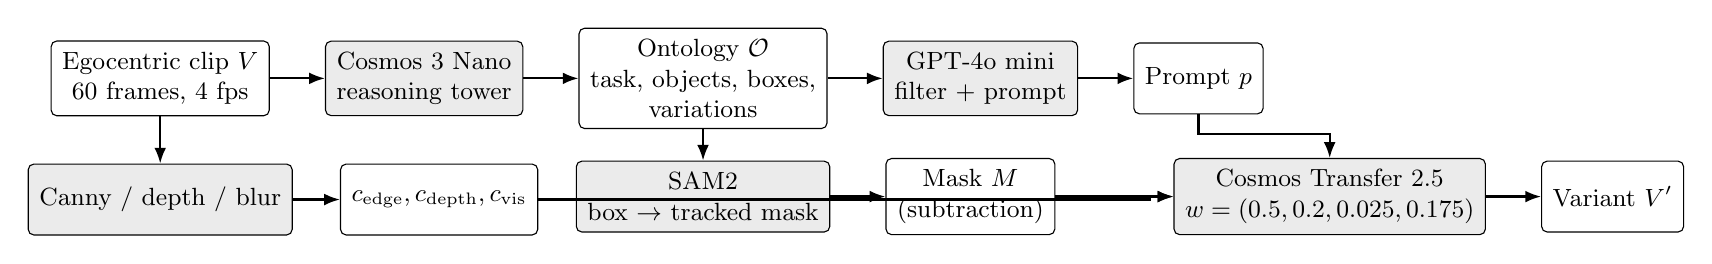
\begin{tikzpicture}[
  node distance=4mm and 7mm,
  box/.style={draw, rounded corners=2pt, align=center, font=\small, inner sep=4pt, minimum height=9mm},
  model/.style={box, fill=black!8},
  data/.style={box, fill=white},
  arr/.style={-{Latex[length=2mm]}, thick}
]
\node[data] (clip) {Egocentric clip $V$\\60 frames, 4 fps};
\node[model, right=of clip] (reason) {Cosmos 3 Nano\\reasoning tower};
\node[data, right=of reason] (onto) {Ontology $\mathcal{O}$\\task, objects, boxes,\\variations};
\node[model, right=of onto] (llm) {GPT-4o mini\\filter + prompt};
\node[data, right=of llm] (prompt) {Prompt $p$};
\node[model, below=of onto] (sam) {SAM2\\box $\to$ tracked mask};
\node[data, right=of sam] (mask) {Mask $M$\\(subtraction)};
\node[model, below=of clip, yshift=-2mm] (pre) {Canny / depth / blur};
\node[data, right=of pre, xshift=-1mm] (ctrl) {$c_{\mathrm{edge}}, c_{\mathrm{depth}}, c_{\mathrm{vis}}$};
\node[model, right=of mask, xshift=8mm] (transfer) {Cosmos Transfer 2.5\\$w = (0.5, 0.2, 0.025, 0.175)$};
\node[data, right=of transfer] (out) {Variant $V'$};
\draw[arr] (clip) -- (reason);
\draw[arr] (reason) -- (onto);
\draw[arr] (onto) -- (llm);
\draw[arr] (llm) -- (prompt);
\draw[arr] (onto) -- (sam);
\draw[arr] (sam) -- (mask);
\draw[arr] (clip) -- (pre);
\draw[arr] (pre) -- (ctrl);
\draw[arr] (ctrl) -| ($(transfer.west)+(-3mm,0)$) -- (transfer.west);
\draw[arr] (mask) -- (transfer);
\draw[arr] (prompt) |- ($(transfer.north)+(0,3mm)$) -- (transfer.north);
\draw[arr] (transfer) -- (out);
\end{tikzpicture}%
}
\caption{Pipeline. The ontology produced by the reasoning stage drives both the text prompt and the segmentation mask, so the same structured output decides what changes and what is held fixed. Control weights $w$ are listed in the order edge, depth, vis, seg.}
\label{fig:pipeline}
\end{figure}

\subsection{Notation}
A clip is a frame sequence $V=\{I_t\}_{t=1}^{T}$ with $T=60$ at 4~fps and resolution $854\times480$. The reasoning model $R$ maps the first frame to an ontology $\mathcal{O}=R(I_1)$ containing a task record, a set of objects $\{o_k\}$ with normalized boxes $b_k\in[0,1000]^4$, and for each object a set of candidate variations $\mathcal{U}_k$. A variation $u\in\mathcal{U}_k$ is a short phrase such as ``solid blue matte.'' The prompt writer $L$ maps $(\mathcal{O},u)$ to a text prompt $p$. The segmenter $S$ maps a box and the clip to a tracked binary mask $S(b_k,V)\in\{0,1\}^{T\times H\times W}$. The generator $G$ maps $(V,p,\{c_j\},w)$ to a variant $V'$, where $c_j$ are control videos and $w$ their weights.

\subsection{Reasoning: from clip to ontology}
\label{sec:reason}
We prompt the reasoning tower of Cosmos 3 Nano~\cite{cosmos3,cosmos3nano} (16B parameters total, 8B in the reasoning tower) with the first frame of the clip and a fixed instruction (Appendix~\ref{app:prompt}). The instruction asks for up to ten task-relevant objects, a tight 2D box for each, and an exhaustive enumeration of variation dimensions: color and appearance, material and texture, size and shape, state and position, condition, interaction, and brand and style. It also asks for scene-level variations and for a ``dataset gaps'' block that states what training on this clip alone would miss. The model answers in a fixed JSON schema inside \texttt{<answer>} tags after a free-form \texttt{<think>} block.

Two features of the schema matter downstream. First, each object carries a \texttt{role\_in\_task} field, so a bucket in a cleaning clip is recorded as a waste container, not just as a bucket. The variations the model proposes for it are then conditioned on that role; it suggests label designs and sizes rather than, say, filling it with soil. Second, each object carries \texttt{robustness\_gaps} with \texttt{common\_failure\_modes}. For the bucket clip these include the bucket slipping and tipping over. Those are action-level variations and we route them away from the appearance renderer (Sec.~\ref{sec:action}). The exhaustiveness instruction is why the raw proposal count is high: the model returns more than 100 candidates per clip, and 72 on average survive the filter below.

We use the first frame rather than the whole clip because the boxes are needed only to seed the tracker, and the objects present in a 15-second household clip rarely change.

\subsection{Guidance: prompt and mask}
\label{sec:guidance}

\paragraph{Prompt writing and filtering}
GPT-4o mini~\cite{gpt4omini} receives the full ontology and is asked to produce prompts for every variation that passes six plausibility checks (Appendix~\ref{app:filter}): the material must bear the task's contact forces, the object must fit the scene, the material must belong in that kind of room, the behavior must be physically possible, the lighting must match the time of day and room, and the object must be one that could plausibly be there. Rejected variations are dropped silently; each accepted one carries a one-line rationale. On average 72 variations per clip survive out of more than 100 proposed. For an accepted variation a second instruction (Appendix~\ref{app:writer}) writes the Transfer prompt. We found three rules, by trial on the bucket clip, that make the rendered output follow the prompt, and the instruction encodes them:
\begin{enumerate}
    \item State the target attribute two or three times in different phrasings and name the material, not just the color: ``smooth matte blue finish'' rather than ``blue.'' The prompt in Appendix~\ref{app:prompts} names the blue countertop three times.
    \item Name every object that must stay unchanged, with ``retain their original appearance,'' and describe lighting and camera as they are in the source.
    \item Describe the result as a scene, not as an edit, in under 300 words. ``A person cleaning a solid blue countertop'' rather than ``change the countertop from white to blue.''
\end{enumerate}
Rule 3 matches how Transfer was trained: its text conditioning is a caption of the output video, not an instruction. Rules 1 and 2 are heuristics against a model that otherwise under-commits to the change or over-applies it. Sec.~\ref{sec:leakage} measures how well Rule 2 holds, and the answer is: only partly.

\paragraph{Mask construction}
\label{sec:mask}
The region to recolor overlaps with objects that must not change: the bucket, the paper towels and the hand all sit on the countertop. We build the mask by subtraction. SAM2~\cite{sam2} takes the surface box $b_{\mathrm{surf}}$ and returns a tracked surface mask that includes whatever lies on the surface. It takes each object box $b_k$ and returns a tracked object mask. The final mask is
\begin{equation}
    M_t = S(b_{\mathrm{surf}},V)_t \;\setminus\; \bigcup_{k} S(b_k,V)_t ,
    \label{eq:mask}
\end{equation}
computed per frame on SAM2's propagated masks, so $M$ is temporally consistent without a separate tracker. Fig.~\ref{fig:mask} shows the four stages. The boxes are the ones the reasoning stage already produced, so this step adds a segmenter but no new detector.

\begin{figure}[t]
\centering
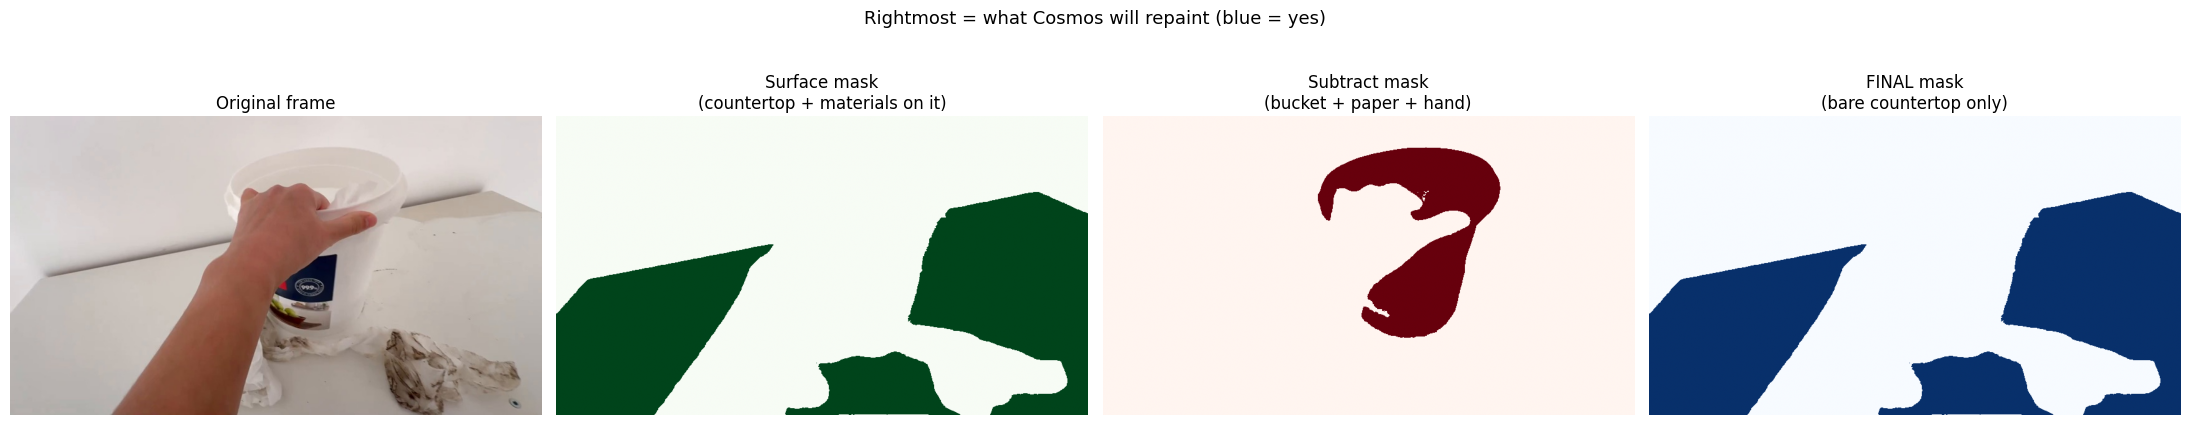
\includegraphics[width=\linewidth]{mask_strip.png}
\caption{Mask construction for the bucket clip. Left to right: original frame; SAM2 surface mask from the countertop box (includes objects on it); union of object masks from the bucket, paper and hand boxes; final mask $M$ after subtraction (Eq.~\ref{eq:mask}). Blue marks the pixels the renderer is meant to change.}
\label{fig:mask}
\end{figure}

\paragraph{Control maps}
Three further controls are derived from the source clip by the preprocessors shipped with Cosmos Transfer: a Canny edge video $c_{\mathrm{edge}}$~\cite{canny1986}, a monocular depth video $c_{\mathrm{depth}}$~\cite{depthanything}, and a heavily blurred RGB video $c_{\mathrm{vis}}$ that carries global color and lighting. The mask $M$ is supplied as the segmentation control $c_{\mathrm{seg}}$. It is a control signal, not a hard constraint: the model follows it to the degree set by the seg weight, and nothing in the pipeline forbids change outside $M$. Fig.~\ref{fig:controls} shows all four for one frame.

\begin{figure}[t]
\centering
\begin{subfigure}{0.24\linewidth}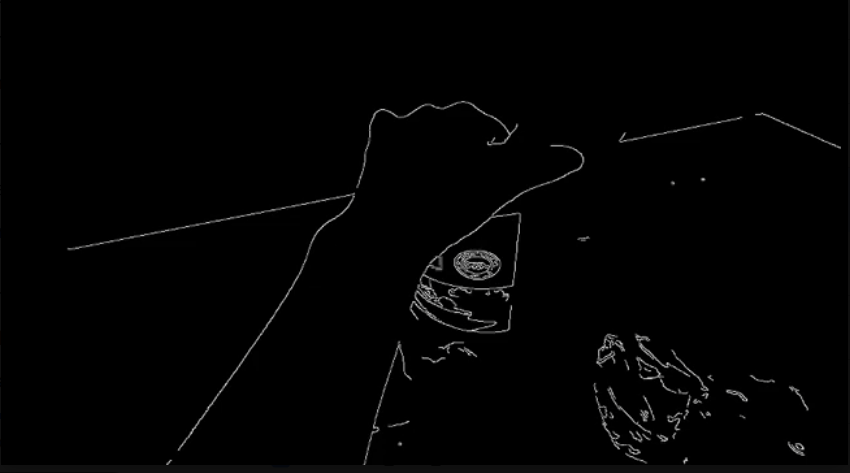
\includegraphics[width=\linewidth]{ctrl_edge.png}\caption{edge}\end{subfigure}\hfill
\begin{subfigure}{0.24\linewidth}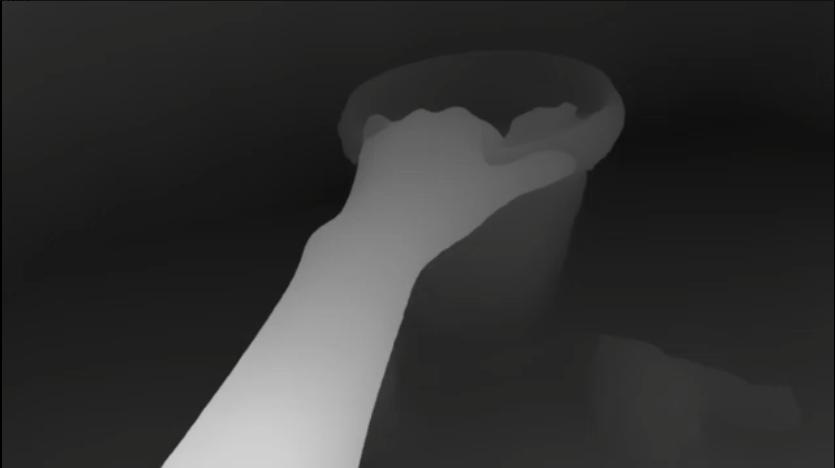
\includegraphics[width=\linewidth]{ctrl_depth.png}\caption{depth}\end{subfigure}\hfill
\begin{subfigure}{0.24\linewidth}
\includegraphics[width=\linewidth]{ctrl_vis.png}\caption{vis}\end{subfigure}\hfill
\begin{subfigure}{0.24\linewidth}
\includegraphics[width=\linewidth]{ctrl_seg.png}\caption{seg ($M$)}\end{subfigure}
\caption{The four control inputs to Cosmos Transfer~2.5 for one frame of the bucket clip. Edge fixes object outlines, depth fixes layout, vis fixes global color and lighting, and the segmentation control carries the subtraction mask.}
\label{fig:controls}
\end{figure}

\subsection{Generation}
\label{sec:generation}
Cosmos Transfer~2.5~\cite{cosmos25,cosmostransfer25} renders $V' = G(V, p, \{c_j\}, w)$ with 35 denoising steps and a guidance scale of 4. The control weights $w$ are the one set of hyperparameters we tuned, and Table~\ref{tab:weights} records the values and the failure that bounds each one. Edge and depth were fixed by failure modes on both sides; the only free choice was how to split the remaining budget between vis and seg. Vis stays near zero because any appreciable weight reasserts the source colors and undoes the recolor. Seg takes the rest. Seeds were not fixed, so a repeated render of the same inputs is not bitwise reproducible. Outputs are 60 frames at $854\times480$ and 4~fps, matching the input.

\begin{table}[t]
\centering
\caption{Control weights for Cosmos Transfer~2.5 and the failure that bounds each. Values are as passed to the model (they sum to 0.9; normalized to 1 they are 0.556, 0.222, 0.028, 0.194). Edge and depth were pinned by failures in both directions; vis and seg share what remains.}
\label{tab:weights}
\small
\begin{tabular}{@{}lS[table-format=1.3]ll@{}}
\toprule
Control & {Weight} & Lower bound failure & Upper bound failure \\
\midrule
edge  & 0.5   & objects lose shape & nothing changes \\
depth & 0.2   & layout drifts & scene flattens to a plane \\
vis   & 0.025 & (none observed) & recolor reverts \\
seg   & 0.175 & edits unlocalized & over-constrained \\
\bottomrule
\end{tabular}
\end{table}

\subsection{Routing action-level variations}
\label{sec:action}
The ontology's failure modes (``bucket tips over'') and state variations are not appearance edits; Transfer preserves the source motion by construction. For these we tried Cosmos Predict2 (2B, Video2World)~\cite{cosmospredict2}, which forecasts frames from a conditioning clip and a text description of what happens next. Sec.~\ref{sec:actionresults} reports the outcome.

\section{Experiments}
\label{sec:experiments}

\subsection{Setup}
\paragraph{Data}
One person recorded 8 egocentric videos of household chores (wiping a counter, folding cloth on a bed, making a bed, wrapping a charger cable at a desk) with a handheld camera, about 10 minutes each. TransNetV2~\cite{transnetv2}, as packaged in Cosmos Curate, split them at shot boundaries into 116 clips, each trimmed to at most 15~s and downsampled to 4~fps and $854\times480$, the input format the Cosmos models expect. The retained set totals about 30 minutes. No robot data is involved; the clips are human demonstrations.

\paragraph{Models and hardware}
Reasoning: Cosmos 3 Nano, reasoning tower~\cite{cosmos3,cosmos3nano}. Prompt writing and filtering: GPT-4o mini~\cite{gpt4omini}. Segmentation: SAM2~\cite{sam2}. Rendering: Cosmos Transfer~2.5~\cite{cosmos25,cosmostransfer25} and Cosmos Predict2 2B Video2World~\cite{cosmospredict2}. All runs were on a single A100 80~GB through Google Colab Pro+. Table~\ref{tab:cost} gives wall-clock per clip.

\begin{table}[t]
\centering
\caption{Per-clip cost on one A100 80~GB (Colab Pro+). Reasoning covers detection, ontology and variation proposals. Transfer time is 35 denoising steps at 31~s each plus about 2~min of control-map preprocessing; Predict2 is 35 steps at 6~s each. The dollar figure is the GPT-4o mini API cost over all 116 clips.}
\label{tab:cost}
\small
\begin{tabular}{@{}llS[table-format=2.1]l@{}}
\toprule
Stage & Breakdown & {Time / clip} & Unit \\
\midrule
Cosmos 3 Nano reasoning & boxes + ontology + proposals & 2.2 & min \\
GPT-4o mini filter + prompt & all 116 clips & {$\approx$\,\$0.12} & total \\
Cosmos Transfer 2.5 render & 35 steps $\times$ 31~s + 2~min maps & 20 & min \\
Cosmos Predict2 2B render & 35 steps $\times$ 6~s & 3.5 & min \\
\bottomrule
\end{tabular}
\end{table}

\paragraph{What was generated}
We ran the reasoning stage on all 116 clips and rendered 64 appearance variants of 10 source clips with Cosmos Transfer, about six variations per clip. The figures in this section show renders of four of those clips (counter wiping, cloth folding, bed making, cable wrapping) under the prompts listed in Appendix~\ref{app:prompts}, chosen because they span the single-surface, multi-texture and shape-collapse behaviors we observed across the set. Two Predict2 renders were made for action-level variation. Evaluation is by inspection of matched frames and by the masked color-difference measurement of Sec.~\ref{sec:leakage}. No policy was trained on the output; Sec.~\ref{sec:limits} returns to this.

\subsection{Appearance variation}
\label{sec:appearance}
Fig.~\ref{fig:bucket} shows the counter-wiping clip and its rendered variant for the prompt ``solid blue matte countertop'' with the bucket, towels, hands and lighting named as preserved. The countertop is blue, the hand pose and the bucket geometry are preserved frame for frame, and the motion is the source motion. The variant also differs from the source in ways the prompt forbade: the towels have become blue cloth, the bucket is grey-blue, the wall has warmed from white to beige, the hand is lighter, and a ceiling fixture appears that was never in the source.

\begin{figure}[t]
\centering
\begin{subfigure}{0.49\linewidth}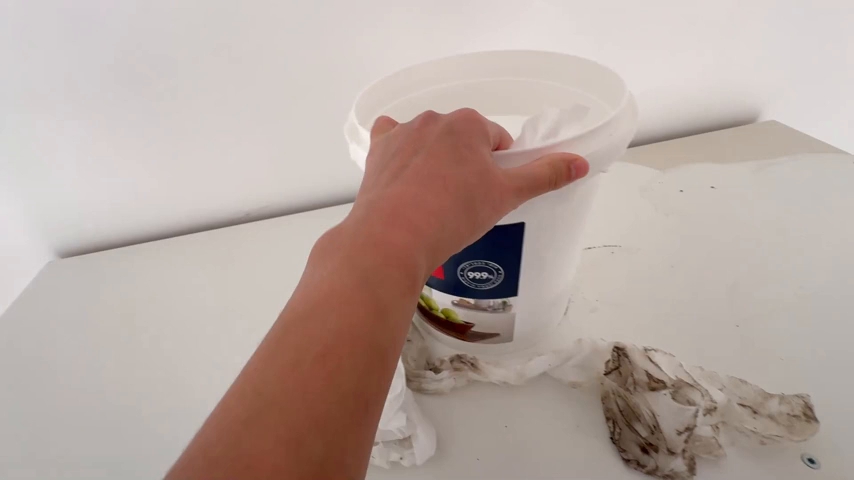
\includegraphics[width=\linewidth]{bucket_orig.png}\caption{source}\end{subfigure}\hfill
\begin{subfigure}{0.49\linewidth}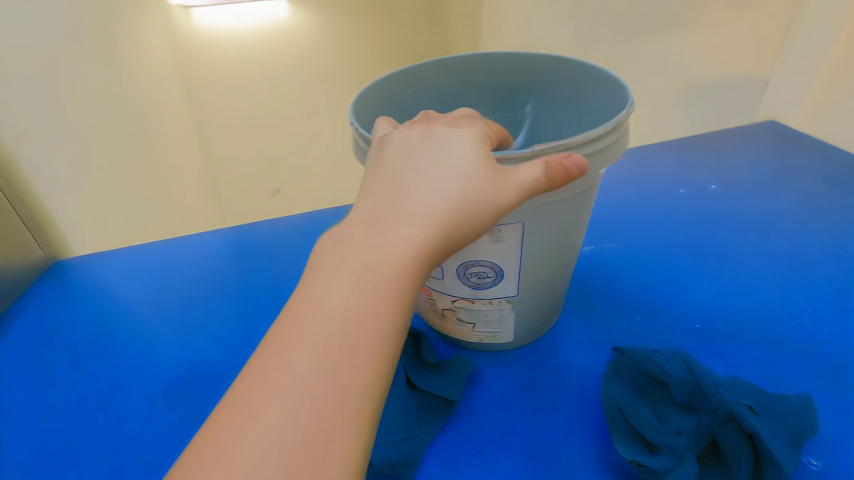
\includegraphics[width=\linewidth]{bucket_gen.png}\caption{variant}\end{subfigure}
\caption{Counter-wiping clip, matched frames. The countertop recolor is the intended edit. The towel, bucket, wall and lighting changes are not; the prompt named each of them as preserved.}
\label{fig:bucket}
\end{figure}

Fig.~\ref{fig:pillow} shows the cloth-folding clip. The prompt asked for a cobalt blue blanket on the left of the bed and listed the white cloth, the patterned pillow, the headboard and a brass ornament as preserved. The render turned nearly every surface blue; the pillow patterns survive only as blue-on-blue relief. Hands are preserved. Fig.~\ref{fig:others} shows the remaining Transfer renders. The desk-and-shelf recolor spread blue onto shelf objects and the cable. The rug prompt for the bed-making clip returned a frame with the correct beige bedspread but heavy smearing and a warped hand, the shape-collapse failure in Table~\ref{tab:weights}. In every case the geometry and the hand motion of the source are retained, and in every case color is applied beyond the target.

\begin{figure}[t]
\centering
\begin{subfigure}{0.49\linewidth}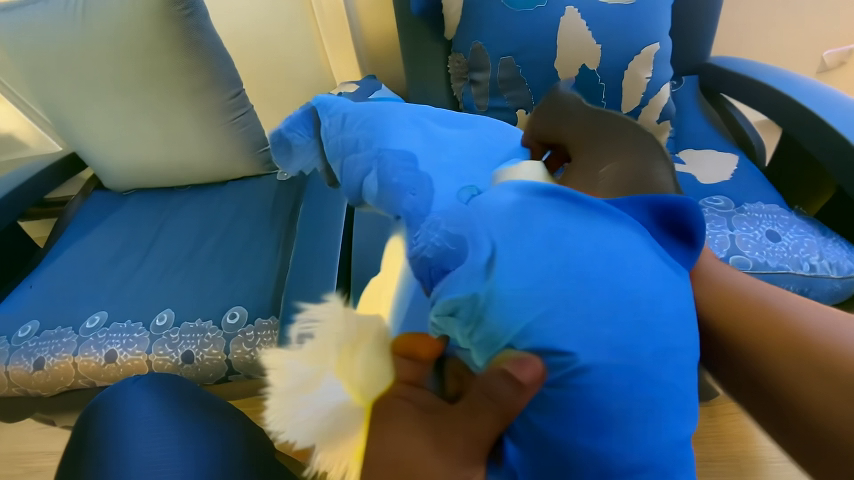
\includegraphics[width=\linewidth]{pillow_orig.png}\caption{source}\end{subfigure}\hfill
\begin{subfigure}{0.49\linewidth}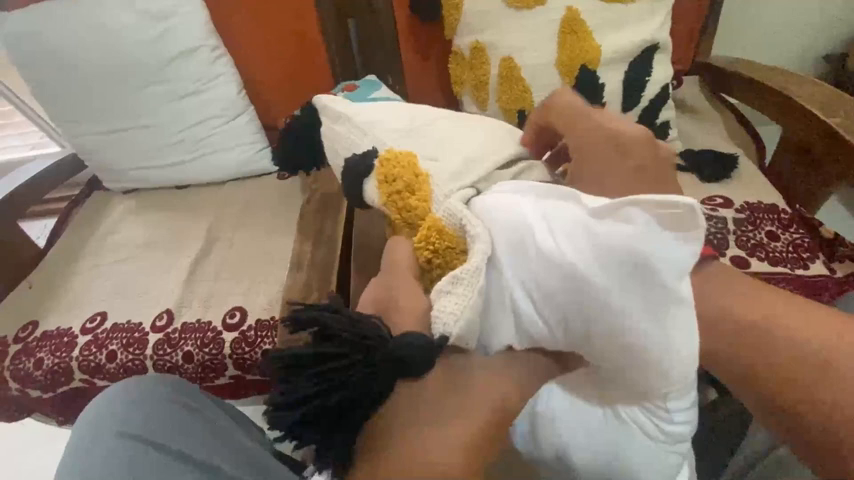
\includegraphics[width=\linewidth]{pillow_gen.png}\caption{variant}\end{subfigure}
\caption{Cloth-folding clip. The prompt targeted a single blanket. The render recolored the cushions, chair and cloth as well. Multi-texture scenes fail more completely than the single-surface case of Fig.~\ref{fig:bucket}.}
\label{fig:pillow}
\end{figure}

\begin{figure}[t]
\centering
\begin{subfigure}{0.23\linewidth}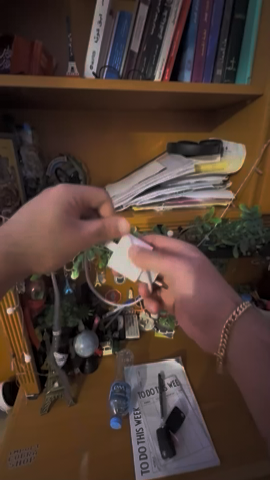
\includegraphics[width=\linewidth]{shelf_orig.png}\caption{desk, source}\end{subfigure}\hfill
\begin{subfigure}{0.23\linewidth}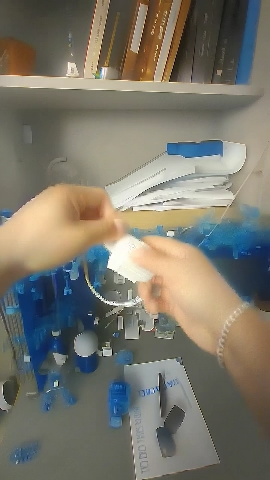
\includegraphics[width=\linewidth]{shelf_gen.png}\caption{blue desk}\end{subfigure}\hfill
\begin{subfigure}{0.48\linewidth}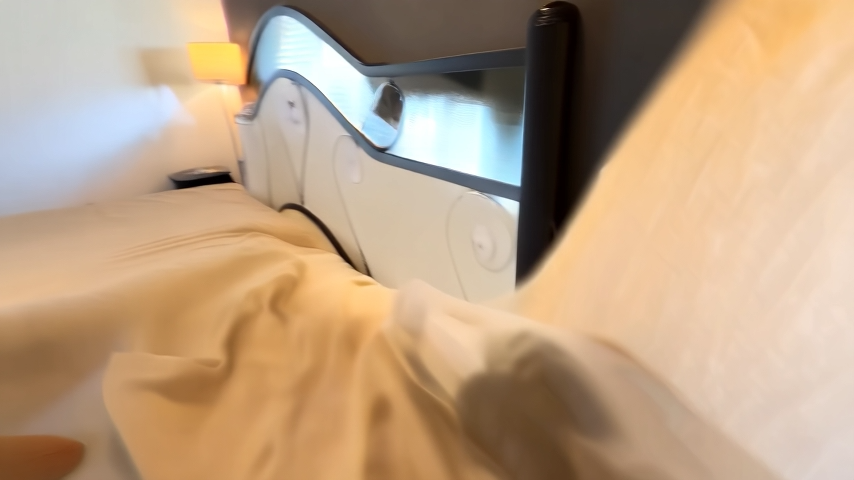
\includegraphics[width=\linewidth]{bed_gen.png}\caption{bed making, navy rug prompt}\end{subfigure}
\caption{Further Transfer renders. (b) Blue leaks from the desk and shelf onto the objects on them. (c) Shape collapse: the bedspread color is right, but surfaces smear and the hand warps.}
\label{fig:others}
\end{figure}

\subsection{Measuring leakage}
\label{sec:leakage}
To put a number on the unintended change, we compare source and variant frame by frame in CIELAB and split the per-pixel CIE76 distance $\Delta E$ by the tracked mask $M$. Pixels inside $M$ are the ones the prompt targeted; pixels outside are the ones it said to preserve. We report the mean over pixels and frames and the fraction of protected pixels whose $\Delta E$ exceeds 10, a difference that is unmistakable to a viewer. Table~\ref{tab:leakage} and Fig.~\ref{fig:leakage} give the result for the counter-wiping clip, the one render for which a usable tracked mask was retained; Sec.~\ref{sec:limits} says what was found for the others.

\begin{table}[t]
\centering
\caption{Masked color difference for the counter-wiping variant, 60 frames. The protected region changes by almost half as much as the target, and nearly all of it changes visibly. Chroma-only distance (a, b channels) shows the change is color, not exposure.}
\label{tab:leakage}
\small
\begin{tabular}{@{}lS[table-format=2.1]S[table-format=2.1]@{}}
\toprule
 & {Target ($M$)} & {Protected ($\bar M$)} \\
\midrule
Mask coverage (fraction of frame) & 0.50 & 0.50 \\
Mean $\Delta E$ & 75.5 & 34.8 \\
Std of per-frame mean $\Delta E$ & 4.0 & 7.2 \\
Mean chroma-only $\Delta E$ & 68.2 & 24.2 \\
Pixels with $\Delta E > 10$ (\%) & {--} & 94.5 \\
Pixels with $\Delta E > 20$ (\%) & {--} & 65.3 \\
\bottomrule
\end{tabular}
\end{table}

\begin{figure}[t]
\centering
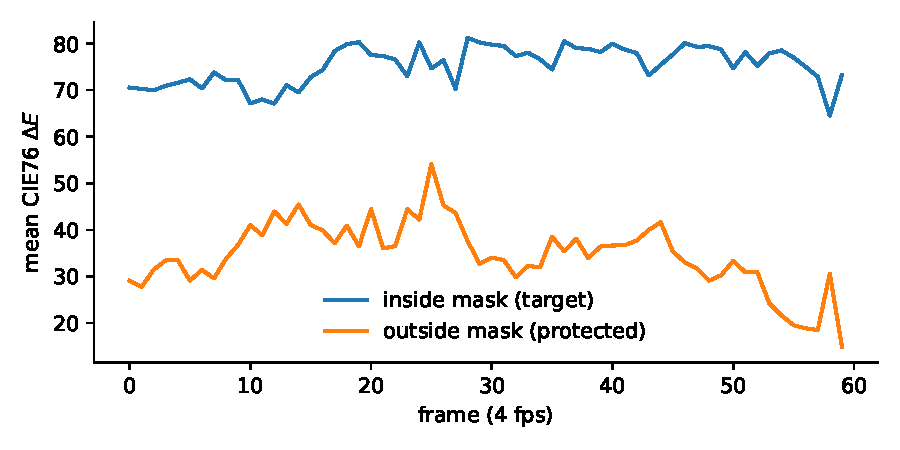
\includegraphics[width=\linewidth]{leakage_per_frame.pdf}
\caption{Per-frame mean $\Delta E$ inside and outside the mask for the counter-wiping variant. The gap is stable across the clip; the protected region never approaches zero.}
\label{fig:leakage}
\end{figure}

\begin{figure}[t]
\centering
\begin{subfigure}{0.32\linewidth}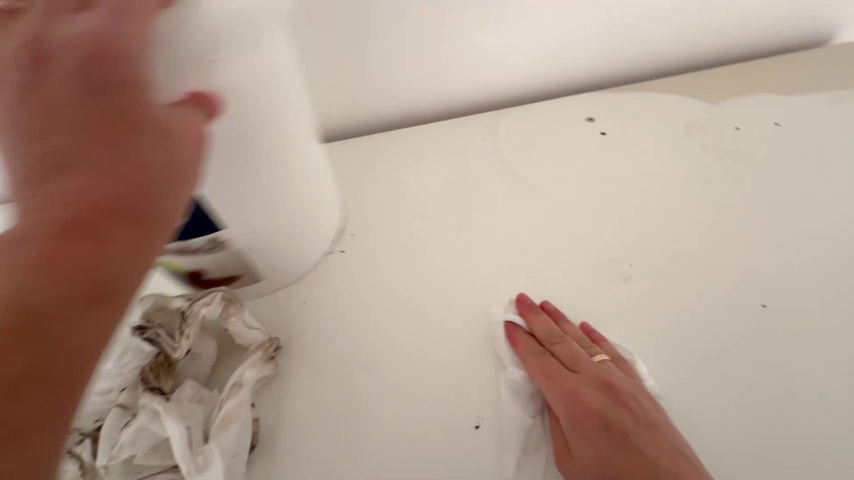
\includegraphics[width=\linewidth]{bucket_orig_f30.png}\caption{source, $t{=}30$}\end{subfigure}\hfill
\begin{subfigure}{0.32\linewidth}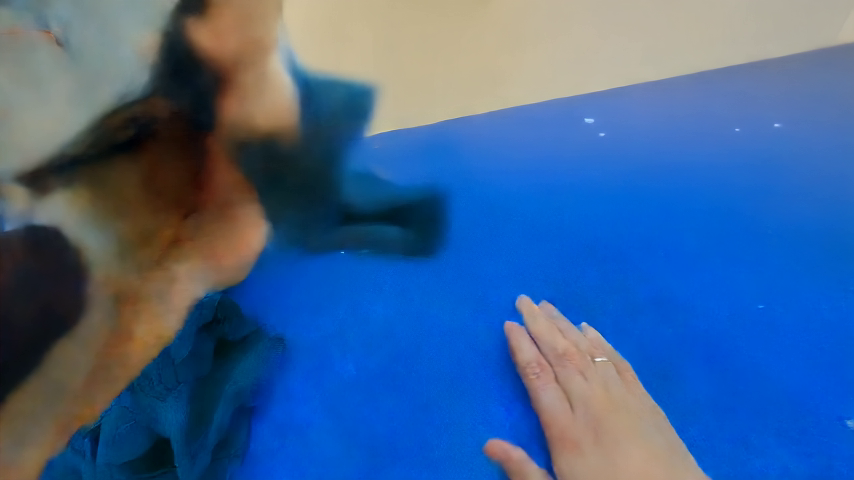
\includegraphics[width=\linewidth]{bucket_gen_f30.png}\caption{variant}\end{subfigure}\hfill
\begin{subfigure}{0.32\linewidth}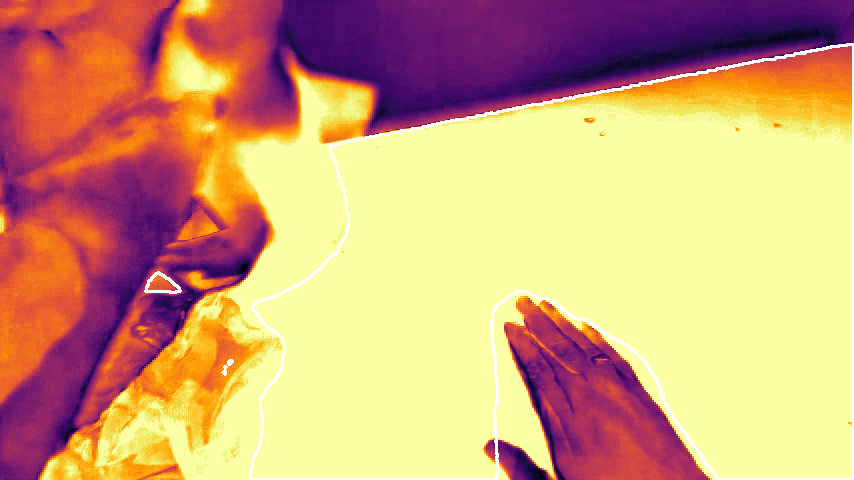
\includegraphics[width=\linewidth]{leakage_heatmap_f30.png}\caption{$\Delta E$}\end{subfigure}
\caption{Spatial distribution of change at frame 30. The white contour is the mask boundary. The towels and bucket (left, outside the mask) change nearly as much as the countertop; the wall (top) changes less but not negligibly.}
\label{fig:heatmap}
\end{figure}

The target region moved by a mean $\Delta E$ of 75, so the recolor itself worked. The protected region moved by 35, and 95\% of its pixels moved by more than 10. The chroma-only columns rule out a mere exposure shift. Fig.~\ref{fig:heatmap} shows where: the towels and bucket, directly adjacent to the target, change almost as much as the target does, and the wall changes less but visibly. With the segmentation control at weight 0.175 and the prompt's preservation clause, the pipeline had two soft mechanisms for containment and neither was sufficient.

\subsection{Control-weight sensitivity}
Table~\ref{tab:weights} summarizes the sweep on the counter-wiping clip. We did not grid-search; each weight was moved until a failure appeared and backed off. Three observations carry over to other clips. Edge weight is the dominant term and is bounded on both sides within a narrow band. Vis must be near zero for any recolor, because the vis branch conditions on the source colors and directly opposes the prompt. Guidance scale trades prompt adherence against realism. At 2 and 3 the model often ignored the variation or applied it weakly; above 5 it followed the prompt and lost the scene, producing frames that no longer read as the same room. All reported renders use 4. We did not find a setting that recolored the target fully and left the protected region unchanged.

\subsection{Action-level variation}
\label{sec:actionresults}
Two action variations from the ontology were attempted with Cosmos Predict2 (35 steps, $848\times480$, 93 frames at 16~fps, seed derived from a hash of the prompt identifier): winding a charger cable around its block one loop at a time with the block held fixed, and a sheet of paper on the desk rotating 90 degrees while three objects on it stay in place (Appendix~\ref{app:prompts}). Both prompts are deliberately specific about what moves, what stays fixed, and how the moving part stays physically attached; the cable prompt even points the model at the input frames as the reference motion. In both renders the forecast frames reproduce the conditioning scene with no visible motion of the cable or the paper (Fig.~\ref{fig:predict}). The model held the scene stable, which is a form of success for a world model, and did not perform the action, which is the only thing we asked of it. We did not fine-tune Predict2; Sec.~\ref{sec:limits} discusses why that is the natural next step.

\begin{figure}[t]
\centering
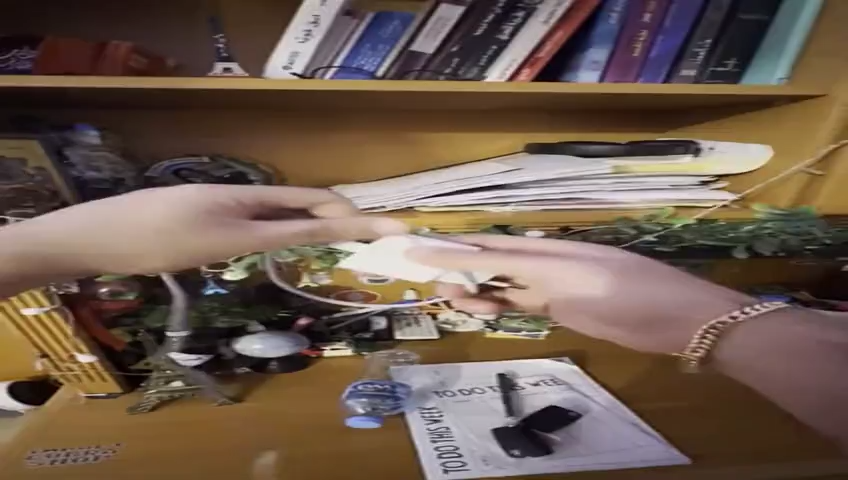
\includegraphics[width=0.45\linewidth]{cord_predict.png}
\caption{Cosmos Predict2 output for ``wrap the cable'' at the last forecast frame. The scene is reproduced; the cable has not moved.}
\label{fig:predict}
\end{figure}

\subsection{Cost of scaling}
Given the per-clip figures in Table~\ref{tab:cost} and 72 admissible variations per clip from Sec.~\ref{sec:reason}, rendering every variation for every clip would produce $116\times72 = 8{,}352$ variants at about 2{,}800 A100-hours. The 64 we rendered took about 21 GPU-hours. The reasoning and filtering stages are negligible by comparison (a few hours and under a dollar). The render is the entire cost, and it is the stage whose output is not yet contained.

\section{Discussion and Limitations}
\label{sec:limits}

Everything in Sec.~\ref{sec:experiments} is about the rendered video. Nothing is about a robot. The claim that appearance variants improve policy generalization is the premise of this work, not a result of it, and the honest reading of the leakage measurement is that the variants we can make today would teach a policy that countertops, towels and buckets change color together. Training a policy on these variants and measuring held-out success is the experiment that decides whether the pipeline is useful, and we have not run it.

The containment failure has a specific cause: the mask entered the renderer only as a segmentation control at weight 0.175, which biases generation toward the mask layout but does not forbid change outside it, and the prompt's preservation clause is a request, not a constraint. Cosmos Transfer~1 supports spatiotemporal control-weight maps, and a hard inpainting formulation that composites source pixels back outside $M$ is trivial to add after the fact. We expect either to cut the protected-region $\Delta E$ by a large factor. We did not do this before the submission deadline, and the measurement in Sec.~\ref{sec:leakage} is the baseline against which that fix should be judged.

The leakage measurement covers one render because the tracked masks retained for the desk and cloth-folding runs are almost empty: under 1\% and about 2\% of the frame respectively, against roughly half the frame for the furniture and blanket regions they were meant to cover. If those are the masks Transfer received, SAM2's propagation collapsed on those clips and the segmentation control carried no information, which would account directly for the whole-frame recoloring in Figs.~\ref{fig:pillow} and~\ref{fig:others}b. We have not yet confirmed whether they are the masks used or a later export, so we report the observation and not the conclusion. Either way, a pipeline that depends on a tracked mask needs a check on mask coverage before rendering, and ours did not have one.

The ontology itself is not fully reliable. For the counter-wiping clip it named the task ``disposing of crumpled paper into a bucket'' when the recording was of wiping, and it listed ``bucket cannot be opened'' as a failure mode for an open bucket. The filter stage exists to catch entries like these, but we have not measured its precision, and the 72-of-100-plus survival rate is a count, not an accuracy. A reviewer should treat the ontology as a strong proposal generator with an unmeasured error rate.

We compare against no baseline. The natural one is a prompt-level version of domain randomization: sample a color and material at random for the same target object, render with the same controls, and have raters judge plausibility against the ontology-driven variant. That experiment is cheap relative to the renders already done and would test the claim that reasoning yields more plausible variation than randomness. Until it is run, that claim is a hypothesis.

Finally, the dataset is small and homogeneous: one person, one home, eight recordings. The control weights in Table~\ref{tab:weights} were tuned on one clip and checked on three others. We would not expect them to transfer unchanged to outdoor scenes or to robot-arm footage.

\section{Conclusion}
A reasoning world foundation model can turn a single egocentric clip into a structured list of task-grounded appearance variations in about two minutes, and a multi-control video-to-video model can render any one of them with the source motion intact in about twenty. The render does not stay inside the lines: on our best case the region meant to be preserved changed by almost half as much as the region meant to change, and action-level variation produced no action. Appearance proposal and rendering are solved well enough to build on. Spatial containment is an engineering gap with a known fix we have not yet measured, and action generation is a research gap. Whether appearance diversity alone makes a policy more general, or whether the action gap has to close first, is the question this pipeline now makes it possible to ask.


\appendix
\section{Reasoning prompt and ontology schema}
\label{app:prompt}
The instruction given to the Cosmos 3 Nano reasoning tower, abridged to the schema. The full text is available from the authors.

\begin{lstlisting}
You are an expert robotics training data analyst with precise spatial grounding.
Analyze this egocentric image of a person performing a household task.
Your goals:
1. Identify the most task-relevant objects in the scene (up to 10).
2. Provide a precise 2D bounding box for each object
   ("bbox_2d": [x1, y1, x2, y2], normalized 0-1000).
3. Enumerate EVERY possible variation for synthetic data generation.

OUTPUT FORMAT (JSON):
{ "location": {room_type, setting, time_of_day, lighting_condition, room_style},
  "task": {name, description, phase, action_primitive, difficulty,
           typical_duration_seconds},
  "key_objects": [{ rank, name, bbox_2d, is_primary, role_in_task,
      "current_appearance": {color_description, rgb, hex, material, texture,
                             condition, size_estimate},
      "current_state": {position_on_surface, height_above_surface, orientation,
                        interaction_state, task_completion_phase},
      "variations": {color_and_appearance, material_and_texture, size_and_shape,
                     state_and_position, condition, interaction, brand_and_style},
      "robustness_gaps": {what_robot_must_handle, common_failure_modes, edge_cases} }],
  "scene_variations": {lighting, camera_viewpoint, room_style_and_culture,
                       time_of_day, background_clutter, person_characteristics,
                       task_sequence_variations},
  "dataset_gaps": {what_current_clip_shows, what_is_missing,
                   highest_priority_variations} }

Answer in the following format:
<think> your reasoning </think>
<answer> your JSON here </answer>
\end{lstlisting}

\section{Plausibility filter instruction}
\label{app:filter}
The instruction given to GPT-4o mini together with the ontology JSON. It filters variations and requests structured prompt entries; the entries are then rewritten as free-text Transfer prompts by the instruction in Appendix~\ref{app:writer}.

\begin{lstlisting}
Here is the variation ontology for a household task clip:
{ontology_json}
Generate a comprehensive set of video generation prompts for Cosmos 3.
CRITICAL: The "prompt" field in each prompt entry must be a complete structured JSON object matching the Cosmos 3 caption schema -- NOT a plain text paragraph.
CRITICAL -- PLAUSIBILITY FILTER: Before including any variation, evaluate it against these real-world plausibility checks. REJECT the variation if ANY apply:
1. Material-task incompatibility: The proposed material cannot physically support the task's contact forces (e.g., a glass countertop for heavy scrubbing, a paper shelf holding books).
2. Object-size violation: The proposed object size would not fit the spatial constraints of the scene (e.g., an industrial-sized bucket on a small countertop).
3. Material-environment mismatch: The material would not realistically exist in the environment type (e.g., outdoor gravel flooring in a kitchen, marble countertops in a garage workshop).
4. Physics contradiction: The variation requires physical behavior the real world does not permit (e.g., a towel standing rigid, water flowing upward).
5. Temporal/lighting inconsistency: The proposed lighting contradicts the time of day or environment (e.g., harsh sunset light in a windowless room).
6. Nonexistent or implausible object: The variation introduces an object that would not plausibly be found in this scene type (e.g., a fire hydrant on a bedroom nightstand).
For each variation you INCLUDE, add a one-line "plausibility_rationale" field explaining why this scenario is observable in a real household. For any variation you REJECT, do not include it in the output -- silently skip it.
Prioritize variations that maximize diversity across the robustness gaps identified in the ontology while remaining grounded in real-world household environments.
\end{lstlisting}

\section{Prompt-writer instruction}
\label{app:writer}
The system instruction given to GPT-4o mini to turn an accepted variation into a Cosmos Transfer prompt.

\begin{lstlisting}
You are an expert at writing prompts for NVIDIA Cosmos Transfer 2.5, a video-to-video model that transforms input videos based on text descriptions. Given a scene description and a specific variation to apply, write a detailed prompt that describes the ENTIRE scene as it should appear AFTER the transformation.
Rules:
1. Describe the changed object in vivid detail: color, material, texture, finish.
2. Explicitly state that all OTHER objects retain their original appearance.
3. Describe the lighting and camera angle as they are in the original.
4. Repeat the target color/material 2-3 times in different contexts to reinforce it.
5. Keep the prompt under 300 words.
6. Do NOT use phrases like "transform" or "change" -- describe the scene as if it already looks the way you want.
7. Be specific about materials: "smooth matte blue finish" not just "blue".
Example output format: "The video captures a person cleaning a solid blue countertop in a well-lit indoor kitchen. [...] The bucket and paper towels retain their original appearance. The room is lit by bright, even overhead ceiling lights that illuminate the blue countertop uniformly."
\end{lstlisting}

\section{Generation prompts}
\label{app:prompts}
Prompts written by GPT-4o mini for the Transfer renders in Sec.~\ref{sec:appearance}, followed by the Predict2 prompts of Sec.~\ref{sec:actionresults}.

\paragraph{Counter wiping, blue countertop (Fig.~\ref{fig:bucket})}
\begin{quote}\small
The video captures a person cleaning a solid blue countertop in a well-lit indoor kitchen. The countertop surface is a rich, vivid blue color with a smooth matte finish, clearly visible under the even overhead lighting. The person uses paper towels and a bucket to wipe down the blue countertop surface. The bucket and paper towels retain their original appearance. The walls and surrounding cabinets are neutral colors. The room is lit by bright, even overhead ceiling lights that illuminate the blue countertop uniformly. The camera captures the scene from a close angle, focused on the person's hands and the countertop surface.
\end{quote}

\paragraph{Cable wrapping, blue desk and shelf (Fig.~\ref{fig:others}b)}
\begin{quote}\small
The video captures a person standing at a solid blue painted desk in a well-lit indoor room. The desk surface is a rich, vivid blue color with a smooth matte finish, clearly visible under the even overhead lighting. A matching blue shelf is mounted on the wall above the desk, also painted the same vivid blue. The person holds a white charger cable in both hands and wraps it carefully. The walls of the room are a neutral light color. The room is lit by bright, even overhead ceiling lights that illuminate the blue furniture uniformly. The camera captures the scene from a close angle, focused on the person's hands and the desk surface.
\end{quote}

\paragraph{Cable wrapping, white desk with oak shelf (no figure)}
\begin{quote}\small
The video captures a person standing at a clean, modern desk in a well-lit contemporary indoor room. The desk has a smooth matte white laminate surface with minimalist straight edges and slim tapered legs. A sleek modern floating shelf is mounted on the wall above the desk, made of light natural oak wood with a clear satin finish, clean straight lines, and concealed mounting hardware giving it a seamless floating appearance. The person holds a white charger cable in both hands and wraps it carefully. The walls are painted a soft warm white. The room is lit by bright, even overhead ceiling lights that cast a clean, shadow-free illumination across the furniture surfaces. The camera captures the scene from a close angle, focused on the person's hands and the desk surface.
\end{quote}

\paragraph{Cloth folding, cobalt blanket (Fig.~\ref{fig:pillow})}
\begin{quote}\small
The video captures a person folding a white cloth on a neatly made bed in a well-lit bedroom. A folded blanket rests on the left side of the bed, made of soft fabric in a rich, vivid cobalt blue color with a smooth matte finish. The blue blanket is neatly folded and sits prominently on the white bedding. The white cloth being folded, the decorative pillow with yellow and black patterns, the dark wooden headboard, and the brass decorative item all retain their original colors and appearance. The room is lit by bright, even indoor lighting.
\end{quote}

\paragraph{Cloth folding, chunky cream knit blanket (no figure)}
\begin{quote}\small
The video captures a person folding a white cloth on a neatly made bed in a well-lit bedroom. A folded throw blanket rests on the left side of the bed, made of thick, chunky hand-knitted wool in a warm cream color with a clearly visible cable-knit pattern and a cozy, textured three-dimensional weave. The knitted throw has a soft, plush appearance with visible yarn stitches and a handcrafted rustic aesthetic. The white cloth being folded, the decorative pillow, the dark wooden headboard, and the brass decorative item all retain their original appearance. The room is lit by bright, even indoor lighting.
\end{quote}

\paragraph{Bed making, navy rug (Fig.~\ref{fig:others}c)}
\begin{quote}\small
The video captures a person making a bed by smoothing a beige bedspread in a bright bedroom. On the floor beside the bed is a simple solid navy blue area rug with a flat woven texture and clean straight edges. The bedspread, the person's hands, and the bed retain their original appearance. The room is lit by bright indoor lighting.
\end{quote}

\paragraph{Predict2, paper rotation (Sec.~\ref{sec:actionresults})}
\begin{quote}\small
The video opens with a person standing at a desk in a warmly lit indoor room. On top of the desk, there exists a to do this week paper with 3 black objects lying on top of the paper. In the person's hands, there is a white charger and cable. The left hand holds the cable that is attached to the charger block held in the right hand. As the video progresses, the cable and charger are held still, fully occupying the person's hands. In the second frame, the paper goes from its initial position to a full 90 degrees rotation. After which the frames stay the same as the initial frame. The 3 black objects maintain their relative position on the paper as the paper rotates with no slipping and sliding off. At the end of the video, the paper has turned 90 degrees to the right from initial positions. The person's hands are still fully occupied with the charger and cable as seen in the initial frame.
\end{quote}

\paragraph{Predict2, cable wrapping (Fig.~\ref{fig:predict})}
\begin{quote}\small
The video opens with a person standing at a desk in a warmly lit indoor room. A white charger cable hangs loosely between the person's two hands. The left hand grips the charger block firmly, holding it completely still, anchoring it in place. The right hand holds the loose end of the cable, ready to begin wrapping. As the video progresses, the left hand remains locked in place as a fixed pivot point. The right hand moves slowly and gradually, looping the cable around the charger block one wrap at a time. The cable moves in a circular like motion around the charger block held in the left hand forming concentric circulars near the charger block which serves as an axis of rotation. For reference, the motion is exactly that of the input frames. The cable follows the rotation of the right wrist exactly, bending and curving through the air as it is dragged in a continuous loop. The cable remains taut between the fingers and the charger block at all times, never going slack or floating free. The cable stays physically connected to both the charger block and the wrapping hand throughout, never detaching or disappearing from view. By the end of the video, the cable is fully wound into a tight coil, every loop visibly connected and continuous. The left hand releases its grip, and the person sets the bundled charger down onto the shelf above the desk.
\end{quote}


\bibliographystyle{splncs04}
\bibliography{refs}

\end{document}
